\documentclass[lettersize,journal]{IEEEtran}
\usepackage{amsmath,amsfonts}
\usepackage{algorithmic}
\usepackage{algorithm}
\usepackage{array}
\usepackage[caption=false,font=normalsize,labelfont=sf,textfont=sf]{subfig}
\usepackage{textcomp}
\usepackage{stfloats}
\usepackage{url}
\usepackage{verbatim}
\usepackage{graphicx}
\usepackage{cite}
\usepackage{listings}
\usepackage{xcolor}
\usepackage{hyperref}
\hyphenation{op-tical net-works semi-conduc-tor IEEE-Xplore}
\usepackage{tabularx}


\begin{document}

\title{PRTP: Partially Reliable Transport Protocol for Internet of Things}

\author{
	\IEEEauthorblockN{Hasan MA Islam, Mehraj Rahman, Mahdin Ohi, Abdullah Sajid}
	
	\IEEEauthorblockA{ \textit{Dept. of Computer Science and Engineering} \\
		\textit{East West University, Dhaka, Bangladesh}\\
	}


\thanks{Contact: shuvra.dev9@gmail.com}
}


\maketitle

\begin{abstract}
This work presents PRTP (Partially Reliable Transport Protocol), a novel transport protocol built on UDP. Although congestion control algorithms like TCP might cause delays, they also provide high-reliability guarantees. On the other hand, while speed is given top priority, UDP has no procedures to guarantee complete data delivery, and the order of messages can be unpredictable. Through a compromise between efficiency and dependability, PRTP seeks to close this gap. PRTP builds upon the raw speed of UDP, adding a touch of partial reliability and orderliness to ensure our precious data nuggets reach their destination safely, even in the untamed frontier of the IoT. It is intended for uses when low latency real-time communication is essential, but total data assurance is not. These restrictions will be addressed in PRTP design by adding methods to improve dependability over UDP. Techniques will be used to guarantee a certain degree of data integrity without requiring TCP's entire dependability. Strategies will be employed to ensure a certain level of data integrity without incurring the overhead of complete reliability offered by TCP.
\end{abstract}

\textbf{Keywords:} Transport layer Protocols, Application layer Protocols, TCP, UDP, PRTP

\section{Introduction}
The proliferation of interconnected devices, including the Internet of Things (IoT), wearables, and even basic mobile phones, heavily relies on low-end devices. These small, resource-constrained gadgets---often powered by batteries---are essential in various contexts. However, their limitations present significant challenges when it comes to communication protocols. The Internet Engineering Task Force (IETF) has identified several hurdles to address before a new transport protocol can achieve widespread adoption, even if it initially seems like a perfect solution. The IETF develops protocol standards that ensure the Internet operates smoothly and adapts to new technologies. Their main focus includes three areas: first, the standardization of protocols like TCP and UDP through Requests for Comments (RFCs); second, the promotion of technological innovation; and third, the careful evaluation of proposed protocol changes. The Internet of Things (IoT) poses a unique challenge. The network landscape is dominated by tiny sensors and wearables that prioritize speed and efficiency. Unlike TCP, which continually monitors network traffic and adjusts data flow, the User Datagram Protocol (UDP) adopts a more streamlined approach. The Transport Layer, acting as the unseen conductor of application-network interactions, is crucial to the expanding realm of Internet applications. This layer balances the needs of applications for reliable delivery or low latency with the requirements of the underlying network, ensuring that data reaches its destination effectively. Established protocols like TCP and UDP have traditionally fulfilled this role. TCP prioritizes assured delivery through acknowledgments and retransmissions, making it suitable for applications where data integrity is critical. However, this emphasis on reliability can lead to increased latency, disrupting real-time communication like online gaming or video conferencing. In contrast, the UDP, the fast messenger, prioritizes speed over reliability, making it suitable for applications that demand low latency.

However, the Internet of Things (IoT) presents a unique challenge. Miniature sensors and wearables dominate the network landscape, prioritizing speed and efficiency. Imagine a wildlife photographer venturing deep into the wilderness, relying on a small, battery-powered device to transmit real-time weather data or track their location. Unlike TCP, the User Datagram Protocol (UDP) takes a more streamlined approach that is a fast-track delivery service inside the network that focuses on sending packets quickly without being slowed down by possible network congestion.

Adding a shim layer on top of UDP is crucial here. We must ensure that this additional layer doesn't unnecessarily increase the packet size by adding too many headers to gain semi-reliability. Our proposed PRTP protocol achieves this by adding minimal headers, and whether anyone wants semi-reliability or not is totally up to them, as this is configurable by turning just a bit on and off. In case of semi-reliability, the receiver needs to send an ACK message. Since UDP doesn't care about delivered packet order, a header is kept to maintain packet sequence, which will help the receiver check for lost packets. The client must acknowledge updates if a reliable flag is on the server. The server will retransmit the update message to the client if no acknowledgment is received within a given timeout. However, the protocol does not guarantee that all messages will be delivered to clients when this reliability flag is turned off. Every packet in PRTP has an optional 32-bit timestamp, which will be utilized for synchronization purposes between sender and receiver, as sequence number only tells us if a packet arrived in the intended order without knowing how long a packet has been delayed or if packets are missing entirely. The receiver will drop the packet for significant delays. This is crucial for applications like time-sensitive networking or collaborative tasks. Also, using timestamps can defend against replay attacks where an attacker resends a previously captured packet. Using the timestamp header can mitigate this attack by simply ignoring the packet that is older than the receiver expects; thus, it can mark this as a replay attempt.

Unlike bulky file transfers, tiny data packets from Internet of Things devices (IoT) cause minimal network congestion even during heavy traffic. This makes UDP, a simple protocol, ideal for these battery-powered devices as it prioritizes speed and low power consumption. PRTP builds upon UDP's strengths by offering an optional reliability feature. This ensures data order if needed while keeping the protocol lightweight. Furthermore, PRTP utilizes sequence numbers and timestamps to guarantee order, identify missing data, and prevent security threats. PRTP perfectly balances speed, reliability, and security for data transfer in IoT.

\section{Importance of Bitfield Structure}
Bitfields do save space. They also allow an easier way to set values that aren't byte-aligned. Rather than bit-shifting and using bitwise operations, we can use the same syntax as setting fields in a \texttt{struct}.

Another place where bitfields are common is hardware registers. If you have a 32-bit register where each bit has a certain meaning, you can elegantly describe it with a bitfield. Such a bitfield is inherently platform-specific. Portability does not matter in this case.

\section{Related Works}
Transport layer protocols are the primary focus for Internet of Things (IoT) devices, offering essential services such as reliable data transfer, flow control, and congestion handling \cite{Shang2016Challenges}. IoT devices are resource-constrained and vary widely, therefore, appropriate transport protocols are essential to confirm efficient communication and data transmission \cite{Liri2018Robustness}. In the context of IoT, conventional transport layer protocols (UDP, TCP) have often encountered issues. While TCP’s overhead and latency constrain devices with limited resources and time-sensitive contexts for data transformation, UDP’s unreliability makes it improper when data integrity is crucial \cite{Shang2016Challenges}. Specifically designed transport layer protocols are needed for this ambience to attain equilibrium between efficiency and reliability and also resource constraints \cite{Grinnemo2002PRTP}. In this scenario, the Partially Reliable Transport Protocol (PRTP) can be addressed \cite{Grinnemo2002PRTP}.
To overcome the shortcomings of TCP and UDP, many specialized protocols have been developed. One of them is the Partially Reliable Stream Control Transmission Protocol (PR-SCTP). PR-SCTP offers efficiency and reliability by extending SCTP’s basic feature—retransmissions for certain data chunks \cite{Rajiullah2012PRSCTP}. In scenarios where on-time delivery is more vital than assured delivery, this mechanism is especially beneficial. CoAP (Constrained Application Protocol) is also a substitute, especially for devices with limited resources \cite{Shelby2014CoAP}. CoAP adds functionalities like observe options and confirmable messages to provide a dependable connection using UDP underneath. But the need for standardized implementations and addressing security concerns remain challenges in lightweight protocols \cite{Liri2018Robustness}.
MQTT, another protocol, provides reliable message delivery using TCP. Its QoS (Quality of Service) levels and publish-subscribe model are suitable for reliable data exchange \cite{OASIS2013MQTT}. However, MQTT’s reliance on TCP faces performance limitations in terms of connection setup and latency, especially over unstable networks \cite{Fernandez2021QUIC}.
Emerging protocols like QUIC attempt to address these concerns by combining UDP’s speed with TCP’s reliability, also offering encryption and stream multiplexing \cite{Iyengar2021QUIC}. However, QUIC’s complexity and cryptographic overhead make it less feasible for constrained IoT devices \cite{Fernandez2021QUIC}.
This work collectively underscores the significance of developing a transport layer protocol that is both efficient and adaptable to the unique demands of IoT environments, with configurable reliability, minimal header overhead, and adaptability across diverse IoT use cases \cite{Liri2018Robustness}.
PRTP emerges to fill this void by augmenting UDP with optional acknowledgments \cite{Grinnemo2002PRTP}. PRTP achieves a balance not addressed by existing protocols. It offers delivery assurance only when necessary, thereby optimizing both energy use and latency. Thus, PRTP positions itself as a compelling alternative to existing transport layer solutions, especially in dynamic IoT ecosystems \cite{Grinnemo2002PRTP}.


\section{Background Study}
Transport layer protocols are the primary focus for Internet of Things (IoT) devices, offering essential services such as reliable data transfer, flow control, and congestion handling. IoT devices are resource-constrained and vary widely, therefore, appropriate transport protocols are essential to confirm efficient communication and data transmission. In the context of IoT conventional transportation layer protocols (UDP, TCP) have often encountered issues. While TCP's overhead and latency constraints devices with limited resources and time sensitive context for data transformation, UDP's unreliability makes it improper when data integrity is crucial. Specifically designed transport layer protocols are needed for this ambience to attain equilibrium between efficiency and reliability and also resource constraints. In this scenario the Partially Reliable Transport Protocol (PRTP) can be addressed.

To overcome the shortcomings of TCP and UDP many specialized protocols have been developed, one of them is Partially Reliable Stream Control Transmission Protocol (PRT-SCTP). PR-SCTP offers efficiency and reliability by extending the SCTP's basic feature retransmissions for certain data chunks. In the scenario where on-time delivery is more vital than assured delivery can benefit most from this mechanism. CoAP (Constrained Application Protocol) is also a substitute especially for devices with limited resources. CoAP adds functionalities like observe options and confirmable messages to provide a dependable connection using USP underneath. But the need for standardized implementations and addressing security concerns are the challenges which remain in lightweight protocols. 

MQTT, another protocol providing reliable message delivery using TCP. Its QoS (Quality of Service) level and publish-subscribe model is suitable for reliable data exchange. However, MQTT's reliance on TCP faces performance limitations in terms of connection setup and latency, especially over unstable networks.

Emerging protolcs like QUIC attempt to address these concerns by combining UDP's speed with TCP's reliability, also having encryption and stream multiplexing. However QUIC's complexity and cryptographic overhead make it less feasible for constrained IoT devices.

This work collectively underscores the significance of developing a transport layer protocol which is both efficient and adaptable to unique demands of IoT environments with configurable reliability, minimal header overhead and adaptability across diverse IoT use cases.

PRTP emerges to fill this void, by augmenting UDP with optional acknowledgments. PRTP achieves a balance which are not addressed by existing protocols. It offers delivery assurance only when necessary, thereby optimising both energy use and latency. Thus, PRTP positions itself as a compelling alternative to existing transport layer solutions, especially in dynamic IoT ecosystems.

\section{System Architecture}
% Insert architecture figure here
\begin{figure}[htbp]
    \centering
    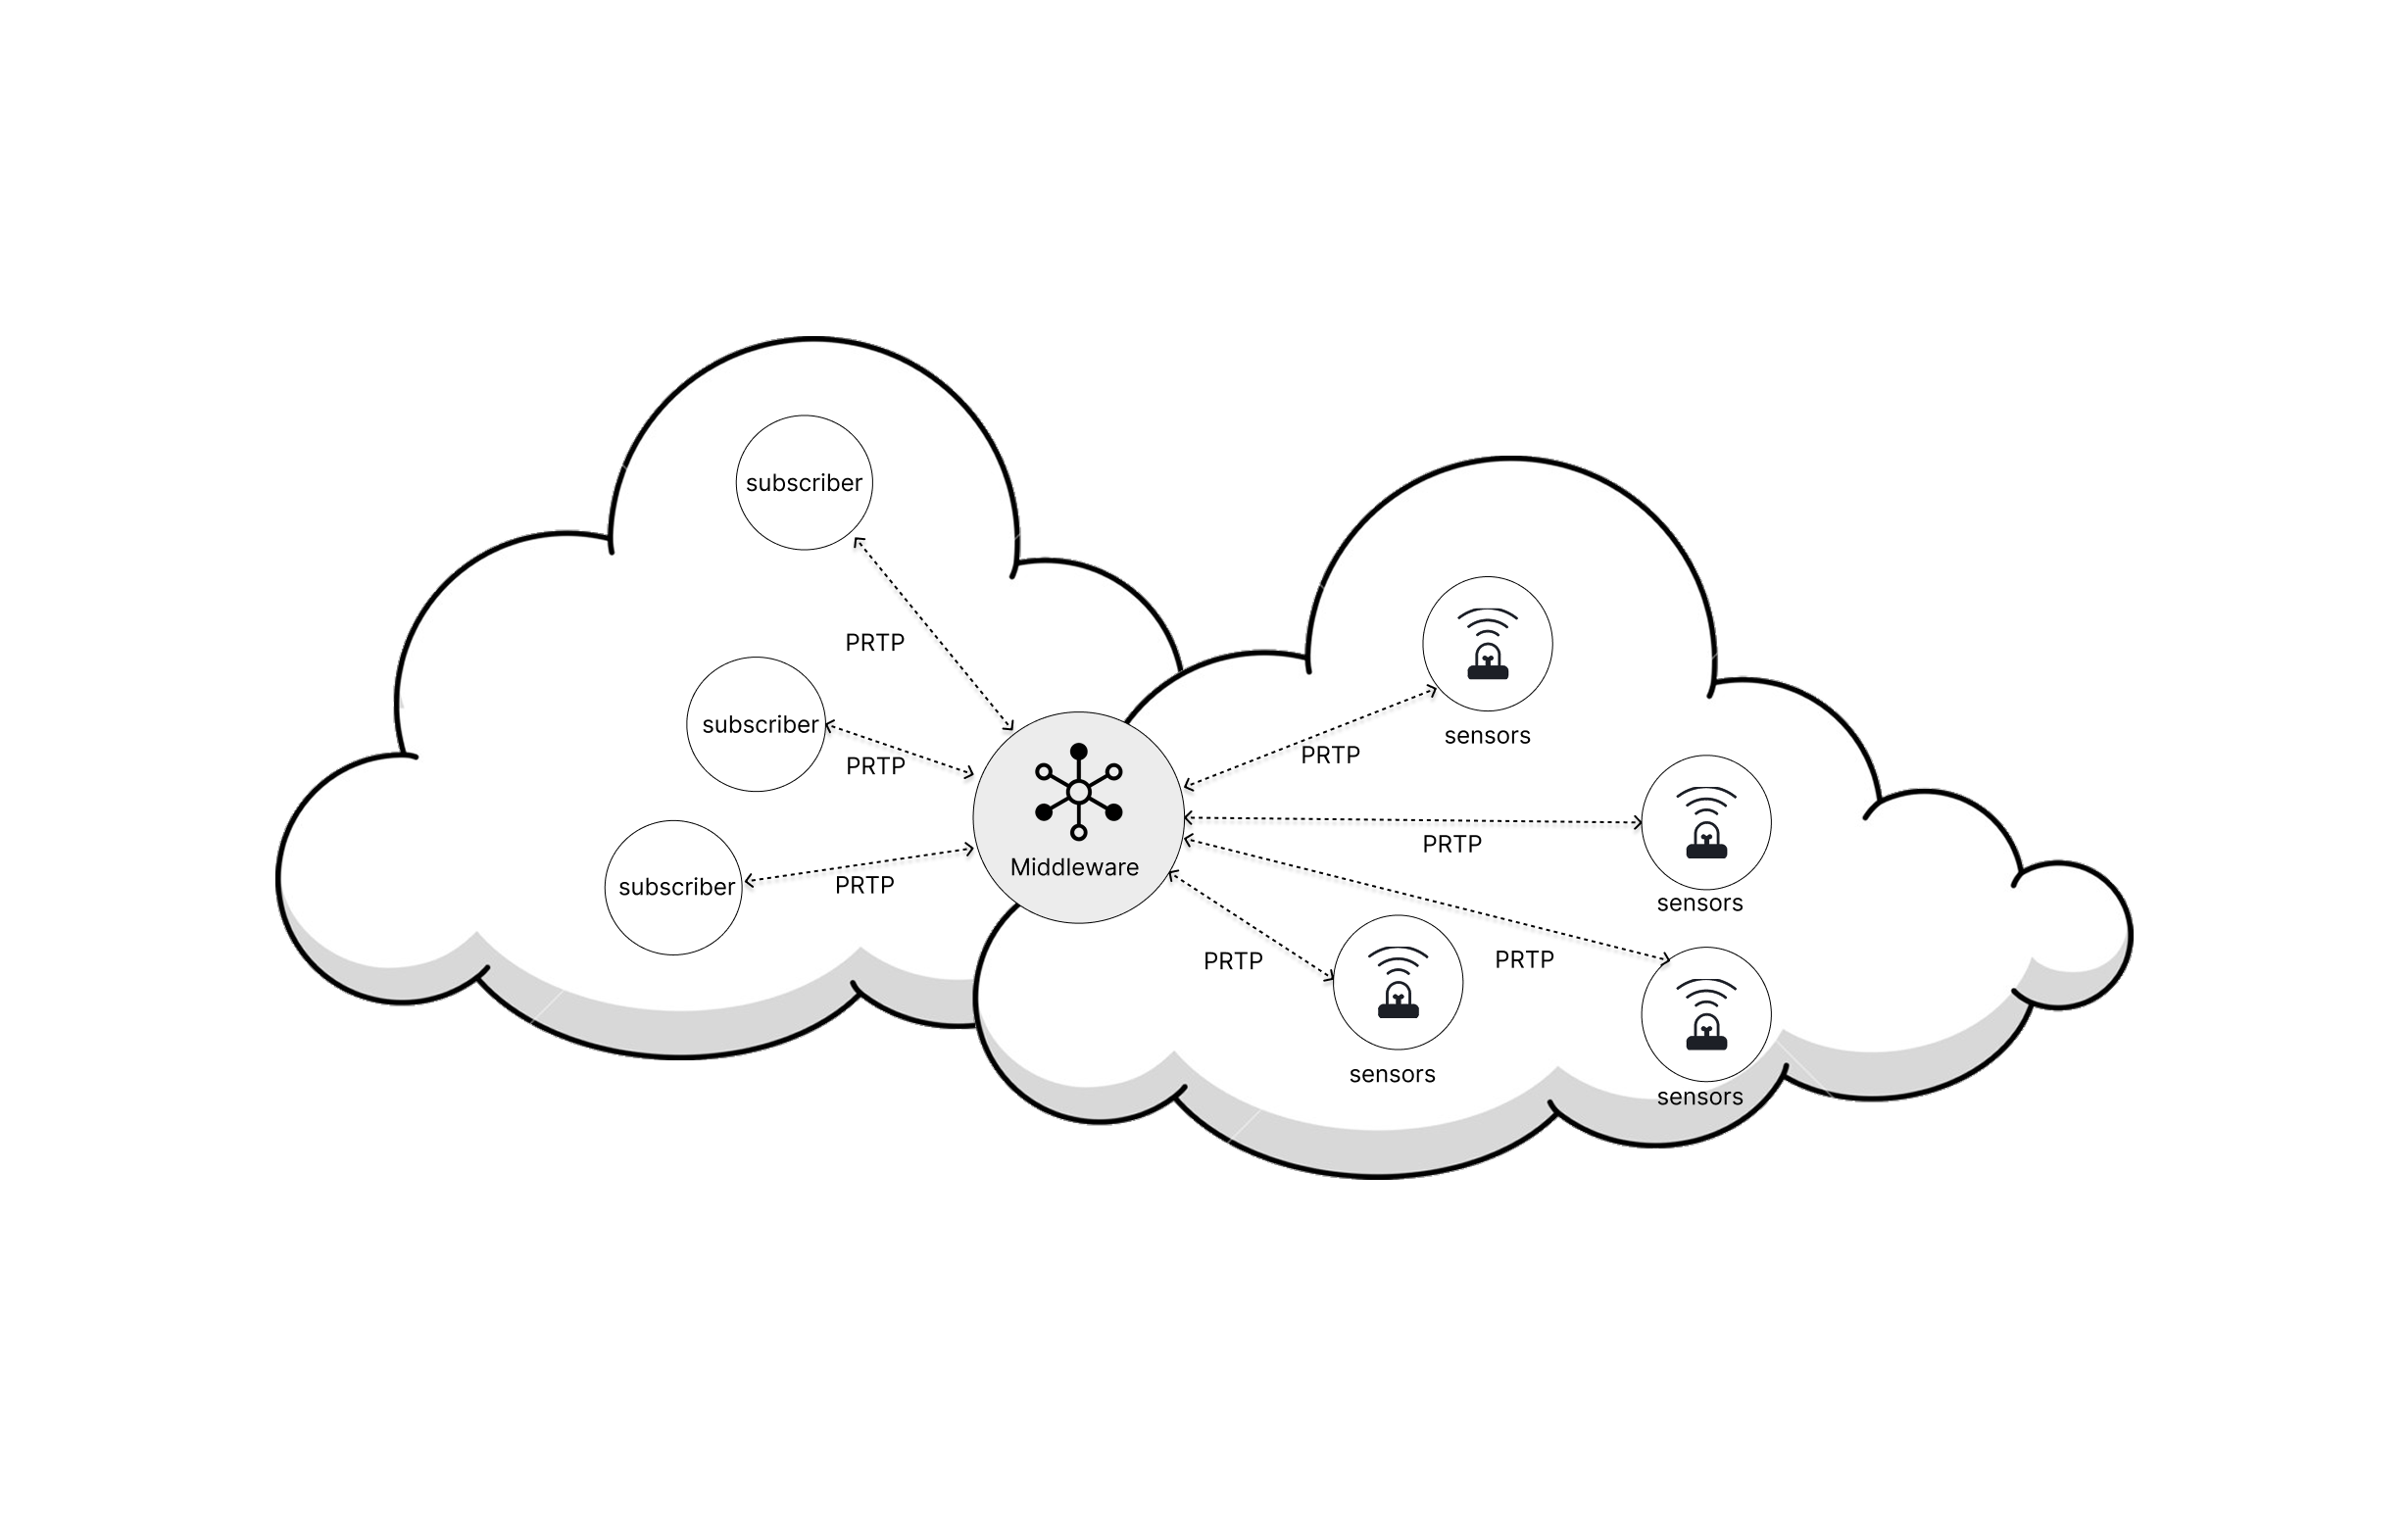
\includegraphics[width=0.8\columnwidth]{Figure/architecture.png}
    \caption{Proposed Publish-Subscribe IoT Architecture}
    \label{fig:iot_architecture}
\end{figure}

\section{Methodology}
The Internet of Things (IoT) paradigm envisions a world where numerous resource-constrained devices seamlessly connect and exchange data, including sensors, actuators, and wearables. These devices often have processing power, memory, and battery life limitations. To facilitate communication between these devices and the external world, a message broker is a central hub for message exchange. The proposed architecture leverages a publish-subscribe paradigm for communication between resource-constrained IoT devices and the internet world. Sensors act as publishers, generating sensor data and publishing it to a central message broker. Subscribers interested in receiving specific sensor data subscribe to relevant topics or sensors through the broker. The message broker efficiently routes published messages to interested subscribers, ensuring data delivery without requiring direct communication between sensors and subscribers.

% Insert methodology figure here
\begin{figure}[htbp]
    \centering
    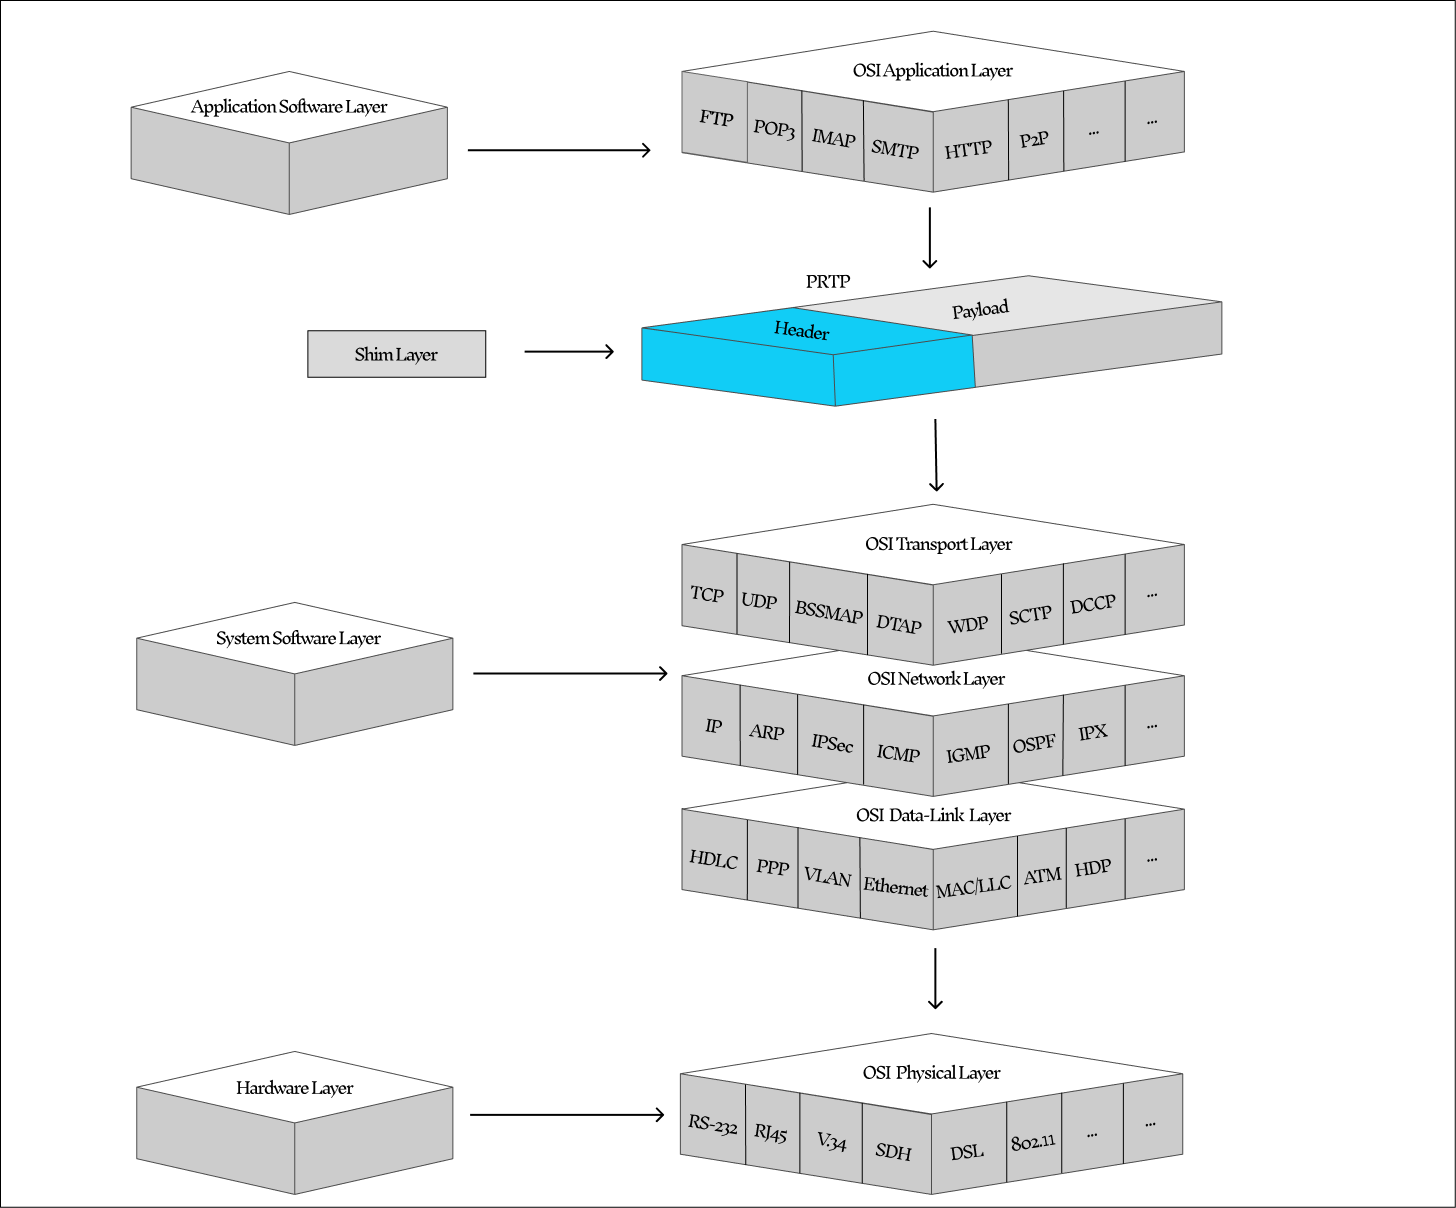
\includegraphics[width=0.8\columnwidth]{Figure/methodology.png}
    \caption{PRTP Methodology Overview}
    \label{fig:methodology}
\end{figure}

To ensure the confidentiality, integrity, and authenticity of data exchanged between sensors and the broker, the Semi Reliable Transport Protocol (SRTP), on top of the UDP protocol, is incorporated into the communication framework. PRTP can be viewed as a two-layered approach, as depicted in Figure~\ref{fig:methodology}:

\textbf{PRTP Shim Layer:} The PRTP Shim Layer sits on top of the User Datagram Protocol (UDP). It handles the asynchronous nature of UDP interactions and provides message types for publish/subscribe communication.

\section{Specification}
\subsection{Message Types}
There are 9 message types currently supported by PRTP:
\begin{itemize}
    \item \textbf{List:} Sent by a subscriber to request a list of all available topics within the network.
    \item \textbf{List Response:} Sent by the broker in response to a List Request.
    \item \textbf{Subscribe:} Sent by a subscriber to indicate interest in a topic.
    \item \textbf{Subscribe Acknowledgment:} Sent by the broker to confirm a subscription.
    \item \textbf{Update:} Sent by sensors to publish new data to the broker.
    \item \textbf{Update Acknowledgement:} Sent by the broker to confirm receipt of an update.
    \item \textbf{Unsubscribe:} Sent by a subscriber to stop receiving data from a topic.
    \item \textbf{Unsubscribe Ack:} Sent by the broker to confirm unsubscription.
    \item \textbf{Keep-alive:} Sent periodically to maintain the connection.
\end{itemize}

\section{PRTP Packet Format}
PRTP message headers act as the compact control center for data exchange processing and error handling within the communication framework, which operates on top of UDP. While designing this packet format to avoid packet fragmentation, it is crucial to understand the minimum MTU (maximum transmission unit) size over the internet. The MTU size represents the largest packet size that can be transmitted without fragmentation. A commonly supported minimum MTU size across many Internet paths is 576 bytes. For IPv6, the minimum MTU is 1280 bytes. To support diverse networks, we have considered 576 bytes as a safe MTU size.

\begin{itemize}
    \item IP Header size = 20 bytes
    \item UDP Header Size = 8 Bytes
    \item PRTP fix header size = 4 bytes
    \item Optional Timestamp header size = 4 bytes
    \item Options header size = variable (0-32 bytes)
    \item PRTP header size with optional header = 8 bytes
    \item Max payload size = 576 - 8 - 20 - 4 = ~544 bytes
    \item Safe Max Payload Size = 500 bytes
\end{itemize}

% Insert packet format figure here
\begin{figure}[htbp]
    \centering
    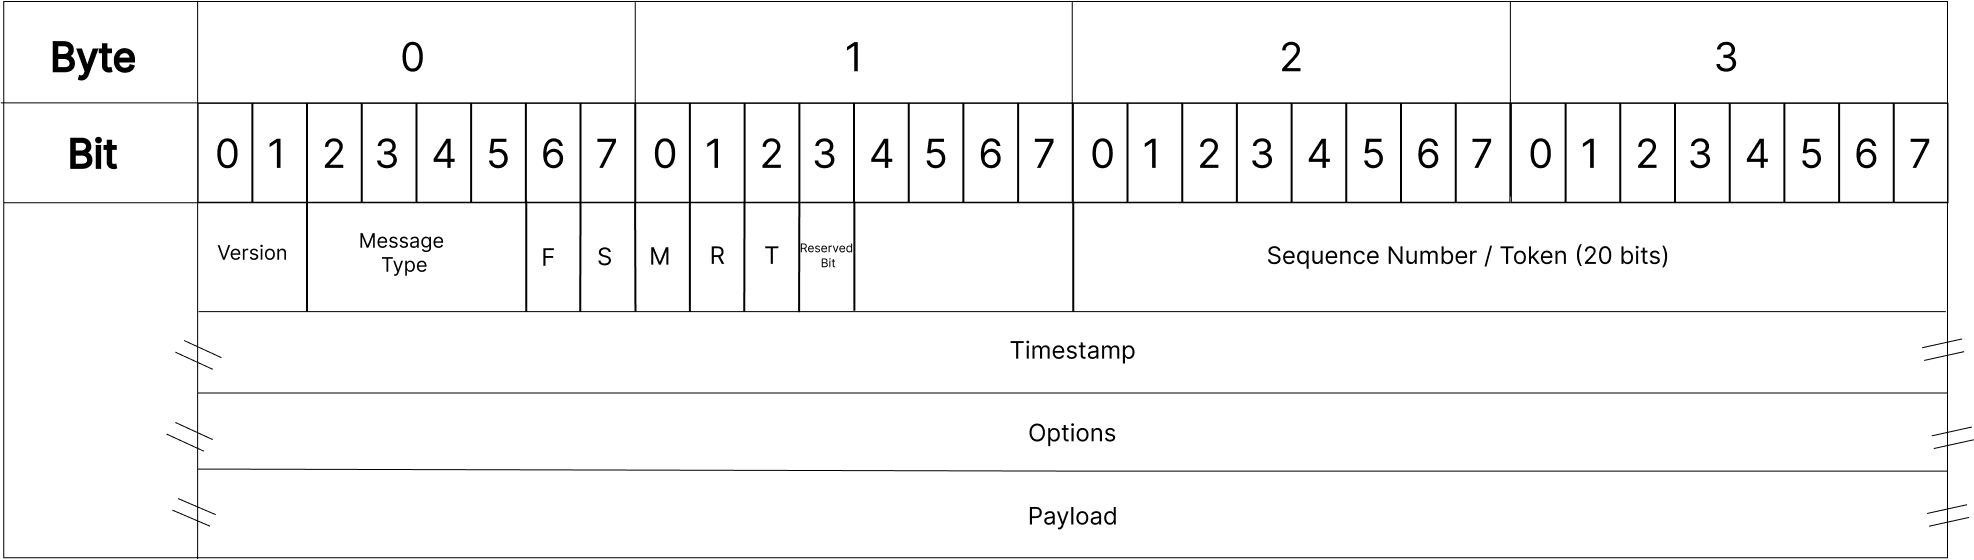
\includegraphics[width=0.8\columnwidth]{Figure/packet_format.png}
    \caption{PRTP Packet Format}
    \label{fig:packet_format}
\end{figure}

\subsection{Header Fields}
\begin{itemize}
    \item Version (2 bits): Protocol version
    \item Message Type (4 bits): Identifies the type of message
    \item F (Fragment Flag, 1 bit): Indicates fragmented payload
    \item S (Start Fragment Flag, 1 bit): Indicates the initial fragment
    \item M (End Marker, 1 bit): Indicates the final packet
    \item R (Reliable, 1 bit): Activates partial reliability
    \item T (Timestamp Flag, 1 bit): Controls inclusion of timestamp header
    \item Reserved Bits (2 bits): Reserved for future use
    \item Sequence Number (20 bits): Sequential message counter
    \item Timestamp (32 bits): Relative timing of packets
    \item Options (0-32 bytes): Optional metadata
    \item Payload (0-500 bytes): Actual data
\end{itemize}

\section{Message Encoding}
\textbf{JSON:} Human-readable, text-based, widely used in web APIs and configuration files. Larger file sizes, slower to parse.

\textbf{BSON:} Binary-encoded, smaller file size, faster to parse, used in databases like MongoDB and high-performance applications.

%\tablespacing
\begin{table}[!t]
\centering
\caption{Comparison Between JSON and BSON Encoding}
\label{tab:json_bson}
\begin{tabular}{|l|p{1.5cm}|p{1.5cm}|}
\hline
\textbf{Features} & \textbf{JSON} & \textbf{BSON} \\
\hline
Format & Text-based & Binary-encoded \\
\hline
Readability & Human-readable & Not human-readable \\
\hline
Data Types & Basic types & Extended types \\
\hline
File Size & Larger & Smaller \\
\hline
Parsing Speed & Slower & Faster \\
\hline
Use Cases & Web APIs, config files & Databases, high-performance apps \\
\hline
\end{tabular}
\end{table}




\section{Operating on Packets}
Each data message is assigned a sequence number. If a message needs to be split into multiple packets, consecutive sequence numbers are assigned to each packet. This helps the receiver order packets correctly and detect any missing packets.

\begin{itemize}
    \item S flag is set to 1 for the first packet of a fragmented message.
    \item F flag is set to 1 for all packets that are part of the fragmented data.
    \item M flag is set to 1 for the last packet of the fragmented data.
\end{itemize}

A process known as fragmentation is employed to transmit large data payloads within the PRTP protocol efficiently. This approach breaks down sizable messages into smaller, more manageable packets. Two key mechanisms are implemented to ensure proper reassembly at the receiver end: sequence numbers and fragmentation flags. Each packet receives a unique sequence number as a numerical identifier within a specific data message. This sequential numbering allows the receiver to correctly order the received packets, even when they arrive out of order due to network fluctuations. In addition to sequence numbers, fragmentation flags provide further context regarding the structure of the message. The "S" flag is set to 1 in the first packet of a fragmented message, notifying the receiver that subsequent packets carrying additional data segments are on their way. Conversely, the "M'' flag is set to 1 in the final packet, acting as an end marker that signals the completion of the fragmented data transmission. Combining sequence numbers and fragmentation flags balances efficiency and scalability within the PRTP protocol. For smaller sensor data payloads, a single packet might suffice, and the receiver can readily identify the final packet based on the presence or absence of the "M'' flag. However, fragmentation is necessary for complex sensors to generate large data volumes. Here, sequence numbers ensure the correct reassembly of the fragmented data at the receiver side, while the "M'' flag efficiently identifies the final fragment, enabling complete data reconstruction. This strategy offers a lightweight and effective solution for data transmission within resource-constrained IoT environments.

\section{Reliability and Timestamps}
To achieve the dual objectives of mitigating replay attacks and determining packet freshness, the protocol employs a 32-bit timestamp field in each packet header. The timestamp is derived from the current time in milliseconds since a fixed epoch (e.g., Unix epoch: January 1, 1970).  The timestamp helps to ensure that old packets cannot be reused maliciously.  The timestamp enables the receiver to assess whether a packet is current or outdated. Additionally, it assists the sender in transmitting the most recent data rather than outdated information if the acknowledgment message from the receiver arrives late in case the reliability flag(R) is turned on. This approach ensures that both the sender and receiver avoid processing stale data. However, there is an option to disable the timestamp header by setting the T (Timestamp) flag to 0. This allows flexibility for use cases where utilizing the timestamp is not necessary. In certain IoT environments, devices may operate under severe resource constraints regarding processing power, memory, and battery life. These devices often perform simple, periodic tasks where the overhead of including and processing timestamps may not be necessary or beneficial. Disabling the timestamp header can be advantageous in such scenarios. Enabling the timestamp header is beneficial to ensure data integrity and freshness, especially when the client devices are not resource-constrained.

Network congestion can cause packets to arrive out of order or be delayed significantly. These delayed packets may contain outdated information in scenarios involving real-time sensor data from IoT devices. Our proposed Semi Reliable Transport Protocol (SRTP) can leverage timestamps within the header to identify and discard these outdated packets. This ensures the receiver processes only the most recent data, improving the overall relevance and timeliness of the information. By comparing the timestamp in the received packet with the current time at the receiver, PRTP can determine if the data is recent enough to be useful. This eliminates the need for the receiver to process and act upon stale information. Timestamps add an extra layer of security. Replaying an old packet with a past timestamp will be easily identified and discarded by the receiver. This reduces the effectiveness of replay attacks, where an attacker attempts to resend a previously captured valid message to disrupt communication. Traditional reliability mechanisms often rely on sequence numbers to detect and eliminate duplicate packets. SRTP's timestamp approach offers a more efficient alternative when the Timestamp flag (T) is on. Instead of maintaining state information about previously received sequence numbers, the receiver compares the timestamp to the current time. This reduces processing overhead, which is particularly beneficial for resource-constrained IoT devices. The effectiveness of timestamp-based methods relies on a certain degree of clock synchronization between sender and receiver. Significant time discrepancies can lead to inaccurate assessments of data freshness. The timestamp header adds a small amount of overhead to each packet.

Additionally, timestamps alone don't guarantee in-order delivery or lossless data transmission. PRTP can combine timestamps with other mechanisms like sequence numbers and acknowledgments (ACKs) to achieve reliable in-order delivery if required by the application. PRTP can utilize reliability flags and sequence numbers along with timestamps. When reliability is crucial, the sender can echo the received timestamp and sequence number in the acknowledgment packet. This confirms successful reception and aids in retransmission if necessary. During acknowledgments, the message type header being set to a specific binary value (ACK) helps the receiver differentiate them from regular data packets. 

To ensure reliable data reception in our proposed protocol, we leverage a receiver-side buffer alongside a timer-based strategy for handling missing or delayed packets. Upon receiving a packet, the receiver utilizes its sequence number to locate its designated position within a buffer. This buffer is a temporary storage area, ensuring packets are placed correctly to reconstruct the complete data stream. Each packet residing in the buffer is assigned an associated timer. If the timer for any packet expires before all expected packets arrive, the entire data transfer is deemed a failure. This mechanism safeguards against indefinitely waiting for missing packets that might be lost due to network issues. 

For an IoT protocol where strict reliability is not crucial but occasional retransmissions are necessary to improve the chances of successful communication, it is crucial to strike a balance between ensuring a reasonable level of reliability and avoiding excessive network traffic and power consumption. As we design a lightweight protocol, we allow a maximum of 3 transmissions. This can handle occasional packet loss without causing significant overhead or delays. It is important to remember that UDP does not provide internal mechanisms for congestion management.  When the reliability flag is on, we can use the acknowledgment mechanism to set the initial timeout interval. Utilizing our timestamp header as the timestamp, included in received data, will be echoed on ACK reply to the ender. Thus, we calculate the round trip times by subtracting the timestamp header value from the current timestamp. 

The RTTs of different packets can be different. To avoid erratic behavior due to fluctuations in RTT, estimated RTT is used, as it is the average of recent measurements, not just the current sample RTT.

\begin{equation}
\text{Estimated RTT} = (1-\alpha) \times \text{Estimated RTT} + \alpha \times \text{Sample RTT}
\end{equation}
Where typically, the value of $\alpha = 0.125$

Deviation in RTT, or Dev-RTT, indicates how evenly the RTT is distributed during the measurement. It depends upon the previously estimated RTT and helps find the retransmission time-out.

\begin{equation}
\text{DevRTT} = (1-\beta) \times \text{DevRTT} + \beta \times |\text{Sample RTT} - \text{Estimated RTT}|
\end{equation}
Where typically, the value of $\beta = 0.125$.

Time-out is longer than RTT, but as RTT varies, we need to add some margin, i.e., safety margin. The selection of a time-out value is essential because the longer the value of the estimated RTT, the slower its performance. We will be facing long delays in this case. Similarly, in the case of a minimal value, the connection can be lost before the RTT completes or before the arrival of the response or acknowledgment. So, for safety, we use

\begin{equation}
\text{Time-out Interval} = 4 \times \text{DevRTT} + \text{Estimated RTT}
\end{equation}

\nocite{*}
\bibliographystyle{IEEEtran}
\bibliography{references}

\end{document}
